% ----------------------------------------------------------
\chapter{Diretrizes da Pesquisa}
% ----------------------------------------------------------

\section{Tema}

O tema dessa tese é o estudo das deformações induzidas pelo processo construtivo de túneis profundos em maciços que apresentam comportamento instantâneo e diferido no tempo.

\section{Metodologia}

A metodologia consiste em uma \textbf{abordagem teórica} derivada da mecânica do contínuo cuja solução é obtida de forma \textbf{numérica} através do \textbf{método dos elementos finitos}.

\section{Objetivos}

O \textbf{objetivo principal} desta tese consiste em formular e programar um modelo constitutivo elastoplástico-viscoplástico para analisar as deformações instantâneas e diferidas induzidas pelo processo de escavação em túneis profundos, incorporando a interação tridimensional entre o maciço e o revestimento.

Como \textbf{objetivos secundários} têm-se:

\begin{alineas}
	 

	\item formular e desenvolver um modelo constitutivo capaz de lidar conjuntamente com o comportamento diferido e instantâneo do maciço;
	
	\item generalizar esse modelo constitutivo para análises em estado plano de deformações, axissimetria (uma vez que essas análises são rápidas do ponto de vista computacional e comuns em diversos estudos na literatura) e tridimensional;
	
	\item implementar o modelo constitutivo acoplado através da customização do \textit{software} ANSYS (versão 2021R1) utilizando a subrotina USERMAT;
	
	\item generalizar o modelo constitutivo para reproduzir tanto o comportamento elástico, elastoplástico, viscoplástico e elastoplástico-viscoplástico, com a possibilidade de implementação de diversas leis de comportamento.
	
	\item verificar o modelo constitutivo com soluções analíticas e numéricas (através do programa GEOMEC91) na problemática de túneis profundos.
	
\end{alineas}

% ---
\section{Delimitações}
% ---
Os túneis podem sofrer influência da superfície como, por exemplo, deformações adicionais devido às cargas superficiais, e, inclusive, intervirem nelas e em suas estruturas através de recalques superficiais ocasionados pela execução do túnel. Contudo, apesar da generalidade dos modelos desenvolvidos no presente trabalho, é dado enfoque nos túneis profundos, portanto, \textbf{não é considerada a influência de estruturas superficiais ou recalques na superfície induzidos pela escavação}.

Embora o maciço em que um túnel está imerso possa apresentar descontinuidades, em muitos casos, seu comportamento global pode ser simulado efetivamente como um \textbf{meio contínuo}. Apesar do comportamento complexo do maciço, que é função também de diversas propriedades que variam espacialmente, nesse trabalho é considerado um \textbf{maciço homogêneo e isotrópico}. Em vista disso, o \textbf{maciço é considerado monofásico} com seu comportamento instantâneo e diferido \textbf{modelado fenomenologicamente através de uma lei reológica} elástica, elastoplástica, viscoplástica e elastoplástica-viscoplástica, \textbf{não considerando, portanto, outras abordagens como, por exemplo, as da poro mecânica, as que tratam da influência do fluxo de água ou da temperatura}.

É também sabido que, em geral, o estado de tensões internas em um maciço é extremamente complexo, devido aos movimentos tectônicos, descontinuidades e heterogeneidades. Contudo, as análises e verificações que são feitas nessa tese considera um \textbf{estado geostático-hidrostático de tensões}. De qualquer forma isso não limita a aplicação do modelo constitutivo desenvolvido para os casos em que o estado de tensões é anisotrópico.

A velocidade de escavação e colocação do revestimento é uma variável importante quando se tem fenômenos diferidos no tempo. Essa velocidade depende de diversos fatores relacionados à dificuldade de escavação do maciço e ao cronograma de execução da obra. Contudo, nesse trabalho, apesar da generalidade do modelo, diferentemente da prática usual de execução de túneis, \textbf{a velocidade de avanço da face de escavação é considerada constante}.

Apesar de um túnel poder atravessar um perfil litológico heterogêneo, o que pode exigir um revestimento e técnicas de pré-suporte especializados para cada região, no presente estudo, o \textbf{revestimento consiste em um modelo único de espessura constante} (sem distinção entre revestimento primário e secundário) ao longo de todo o eixo longitudinal do túnel.

Principalmente em escavações não mecanizadas, é comum a frente de escavação apresentar parcializações de modo a estabilizar ou diminuir as deformações dessa zona. Apesar disso, nesse trabalho a \textbf{escavação é feita à seção plena, plana e vertical sem considerar nenhuma técnica ou elemento de pré-suporte}.

Os modelos incorporados no programa são: \textbf{elástico, elastoplástico, viscoplástico e elastoplástico-viscoplástico}. Para o maciço é considerado o modelo clássico elastoplástico de Drucker-Prager e o modelo viscoplástico de Perzyna (1966) com a mesma superfície de escoamento do modelo elastoplástico, contudo, não necessariamente com os mesmos valores dos parâmetros. De qualquer forma o modelo permite a implementação de outras superfícies de escoamento. \textbf{Para o revestimento é utilizado o modelo elástico linear}.

A evolução das deformações se dá de forma \textbf{quase-estática}, portanto, não são considerados os termos inerciais (densidade e aceleração) ou excitações dinâmicas (como seria, por exemplo, em uma análise considerando terremotos e explosões). Além disso, é considerada a \textbf{hipótese das pequenas perturbações}.

% ---
\section{Delineamento}
% ---

O trabalho foi realizado através das seguintes etapas:

\begin{alineas}

	\item pesquisa bibliográfica sobre túneis e o tema da tese;
	
	\item pesquisa bibliográfica sobre os modelos constitutivos elastoplásticos e viscoplásticos que são comumente utilizados para modelagem de túneis profundos;
	
	\item pesquisa bibliográfica sobre a formulação e solução do problema no contexto de elementos finitos;
	
	\item desenvolvimento do modelo constitutivo e sua solução numérica considerando o comportamento instantâneo elastoplástico acoplado com o comportamento diferido viscoplástico;
	
	\item generalização do modelo constitutivo para abordar problemas em estado plano de deformações, axissimetria e tridimensional;	
	
	\item implementação do modelo desenvolvido na subrotina responsável pelo modelo constitutivo do \textit{software} ANSYS;	
	
	\item desenvolvimento dos domínios de túneis profundos no \textit{software} ANSYS através da linguagem APDL (\textit{ANSYS Parametric Desing Lenguage});
	
	\item verificação da solução numérica com soluções analíticas e numéricas (através do GEOMEC91);
	
	\item estudo da diferença entre considerar o modelo elastoplástico-viscoplástico em relação a outros modelos mais simples.

\end{alineas}

O organograma da \autoref{organograma} ilustra a relação entre as etapas durante o trabalho.

\begin{figure}[H]
	\begin{center}
		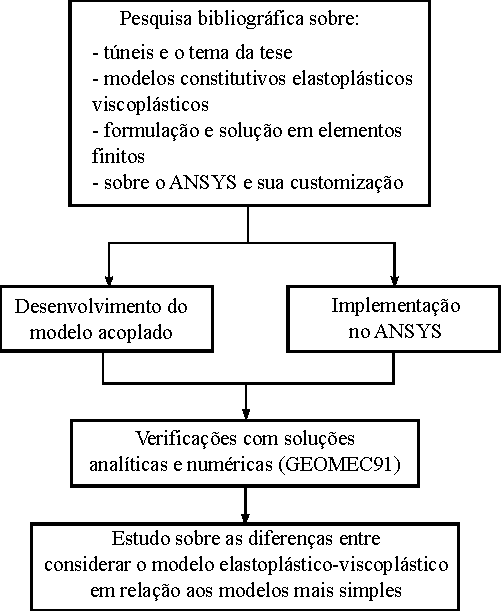
\includegraphics[scale = 1.2]{0201-organograma das etapas da pesquisa.pdf}
	\end{center}
	\caption{\label{organograma}Organograma das etapas da pesquisa}
\end{figure}